\section{}

A round bar is composed of three segments of the same material as shown in Fig. \ref{fig:Q6}. The diameter
is $d$ for the lengths $BC$ and $DE$ and $n\times d$ for length $CD$, where $n$ is the ratio of the two diameters.
Neglecting the stress concentrations, verify that the strain energy of the bar when subjected to
axial load $P$ is
\[
U = \frac{1 + 3n^2}{4n^2} \frac{P^2L}{2AE}
\]
where $A = \frac{\pi d^2}{4}$. Compare the results for $n = 1$ with those for $n = \frac{1}{2}$ and $n = 2$.

\begin{figure}[h]
    \centering
    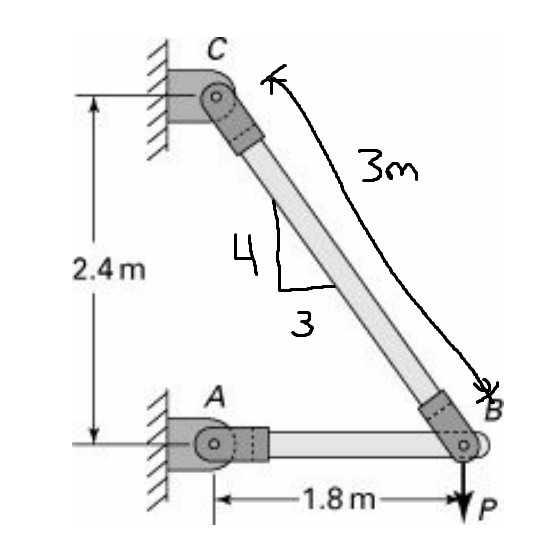
\includegraphics[width=0.5\linewidth]{Questions/Figures/Q6ProblemDiagram.png}
    \caption{Round bar composed of three segments.}
    \label{fig:Q6}
\end{figure}

\textbf{Solution}

The strain energy of the bar segment is given by the integral
\[
U = \int_{L_i}^{L_{i+1}} \frac{P^2}{2AE} dx
\]

The strain energy of the bar is the sum of the strain energies of the three segments:
\[
U = \int_{\text{B}}^{\text{C}} \frac{P^2}{2A_{\text{BC}}} dx + \int_{\text{C}}^{\text{D}} \frac{P^2}{2A_{\text{CD}}} dx 
+ \int_{\text{D}}^{\text{E}} \frac{P^2}{2A_{\text{DE}}} dx
\]

Since the rod is of the same material, $E$ is constant. For segment CD, $A_{\text{CD}} = n^2 A_{\text{BC}} = n^2 A_{\text{DE}}$.
The larger area segment comprises of $L/4$ of the total length. The rest of the rod of cross-sectional area $A$. 
\[
\begin{aligned}
    U &= \int_{0}^{3L/4} \frac{P^2}{2EA} dx + \int_{0}^{L/4} \frac{P^2}{2En^2A} dx \\
    &= \frac{P^2L}{2EA} \bigg|_0^{3L/4} + \frac{P^2L}{2En^2A} \bigg|_0^{L/4} \\
    &= \left(\frac{3}{4} + \frac{1}{4n^2}\right) \frac{P^2L}{2EA} \\
    &= \boxed{\frac{1 + 3n^2}{4n^2} \frac{P^2L}{2AE}} \\
\end{aligned}
\]

For $n = 1, \frac{1}{2}, 2$,
\[
\begin{aligned}
    U|_{n=1} &= \frac{1 + 3(1)^2}{4(1)^2} \frac{P^2L}{2AE} = \frac{4}{4} \frac{P^2L}{2AE} = \boxed{\frac{P^2L}{2AE}} \\
    U|_{n=\frac{1}{2}} &= \frac{1 + 3(\frac{1}{2})^2}{4(\frac{1}{2})^2} \frac{P^2L}{2AE} = \boxed{\frac{7}{4} \frac{P^2L}{2AE}} \\
    U|_{n=2} &= \frac{1 + 3(2)^2}{4(2)^2} \frac{P^2L}{2AE} = \frac{1 + 12}{16} \frac{P^2L}{2AE} = \boxed{\frac{13}{16} \frac{P^2L}{2AE}} \\
\end{aligned}
\]